%%%%%%%%%%%%%%%%%%%%%%%%%%%%%%%%%%%%%%%%%%%%%%%%%%%%%%%%%%%%%%%%%%%%%%%%%%%%%%
%
% Section file included in main project file using \input{}
%
% Assumes that LaTeX2e macros and packages defined in cg_comp.sty are
%   available
%
%%%%%%%%%%%%%%%%%%%%%%%%%%%%%%%%%%%%%%%%%%%%%%%%%%%%%%%%%%%%%%%%%%%%%%%%%%%%%%

 \section{Experimental Estimate of the String Constant\label{sct:exp}}

\red{This section needs to be rewritten.} How do we estimate the spring constant $\kappa$ given by \eqn{kappa_def}? Recall how we introduced this concept in \sct{model_tension}: increasing the tension by a quantity $\Delta T$ causes a shift in the frequency of a guitar string by $\Delta \nu$ in cents. Although we were considering fretted strings when we derived \eqn{error_def}, the terms in that equation can be generalized to describe the case of an open string that has been stretched longitudinally. Suppose that we continue to clamp the string at the saddle and the nut, but that we tighten the tuning gear to stretch that string's length by an amount $\Delta L$. The change in the string's frequency due to the change in the open resonant length is zero, because $L_0 / \gamma_0 L_0 = 1$. The linear mass density of the string is smaller now because there is less material between the saddle and the nut, causing the frequency shift (in cents)
 \begin{equation}
600\, \log_2 \left(  \frac{\mu}{\mu + \Delta \mu} \right) \approx \frac{600}{\ln(2)}\, \frac{\Delta L}{L}\, ,
 \end{equation}
where $L$ is the initial length of the string. Finally, the tension in the string increases by $\Delta T$ due to the elastic properties of the string. Following the discussion in \sct{model_tension}, the corresponding frequency shift  is
 \begin{equation}
600\, \log_2 \left(  \frac{T + \Delta T}{T} \right) \approx \frac{600}{\ln(2)}\, \frac{\Delta L}{L}\, \kappa\, ,
 \end{equation}
where $T$ is the initial tension of the string. Therefore, the total frequency shift of the open string caused by a change $\Delta L$ in the string's length is
 \begin{equation}
\Delta \nu \approx \frac{600}{\ln(2)}\, \frac{\Delta L}{L}\, (\kappa + 1)\, .
 \end{equation}
Solving this expression for the string constant, we find
 \begin{equation}
\kappa = \frac{\ln(2)}{600}\, R - 1\, ,
 \end{equation}
where
 \begin{equation}
R \equiv \frac{L}{\Delta L}\, \Delta \nu
 \end{equation}
is a parameter originally defined by Byers\footnote{Byers expressed this parameter in terms of the fractional frequency shift (in Hertz) as $R = (L/\Delta L) (\Delta f/f) \approx (\ln(2)/1200) (L/\Delta L) \Delta \nu$. Therefore, our dimensionless value of $R$ is larger than Byers' by a factor of about 1730.}~\cite{ref:byers1996cgi,ref:varieschi2010icf}.

It is relatively easy to estimate the value of $R$ for any guitar string with the aid of a simple device that can measure frequency shifts in cents~\cite{ref:pgtweb} and either calipers or a ruler with finely marked graduations. With a fine-point felt pen, make a small mark on the string at some convenient point (say, directly above the first fret). Then tighten that string's tuning gear to increase the frequency by an amount measured using the electronic tuner. (A particularly convenient shift is four half-steps, corresponding to $\Delta \nu = 400$~cents, which will require a stretch of approximate $5 - 6$~mm.)

% \begin{equation}
% \begin{split}
%L_{n \ge 1}(y) &= \sqrt{\left(X_n + \Delta S\right)^2 + (b + c)^2 + y^2} \\
%&\approx X_n + \Delta S + \frac{(b + c)^2 + y^2}{2\, X_n}\, .
% \end{split}
% \end{equation}
%
% \begin{equation}
% \begin{split}
%L^\prime_{n \ge 1}(y) &= \sqrt{\left(X_0 - X_n + \Delta N\right)^2 + b^2 + y^2} \\
%&\approx X_0 - X_n + \Delta N + \frac{b^2 + y^2}{2 \left(X_0 - X_n\right)}\, .
% \end{split}
% \end{equation}
%
% \begin{equation}
% \begin{split}
%Q_n(y) &\approx \frac{1}{2\, X_0} \left[ \frac{(b + c)^2 + y^2}{X_n} + \frac{b^2 + y^2}{X_0 - X_n} - \frac{c^2}{X_0} \right] \\
%&= Q_n(0) + \Delta Q_n(y) \, ,
% \end{split}
% \end{equation}
%where $Q_n(0)$ is given by \eqn{lambda_n_approx}, and
% \begin{equation}
%\Delta Q_n(y) \equiv \frac{1}{2 \left(\gamma_n - 1\right)}\, \left(\frac{\gamma_n\, y}{X_0}\right)^2\, .
% \end{equation}
%
%Following the same approach we used to derive \eqn{quad_shift}, we can derive the change in the total shift due to both resonant length and linear mass density for a transverse displacement $y$. To second order in $y$, we find that
% \begin{equation}
%\Delta \nu_n(y) \approx \frac{600}{\ln(2)}\, \frac{3 - 2 \gamma_n}{2 \left(\gamma_n - 1\right)}\, \left(\frac{\gamma_n\, y}{X_0}\right)^2\, .
% \end{equation}
%We have plotted this expression for the first 12 frets and $y = 5$~mm in \fig{quad_shift_factory}. This shift is quite small compared to the experimental errors we'll obtain in the shifts due to tension, and we ignore it in what follows.
%
% \begin{figure}
%  \centering
%  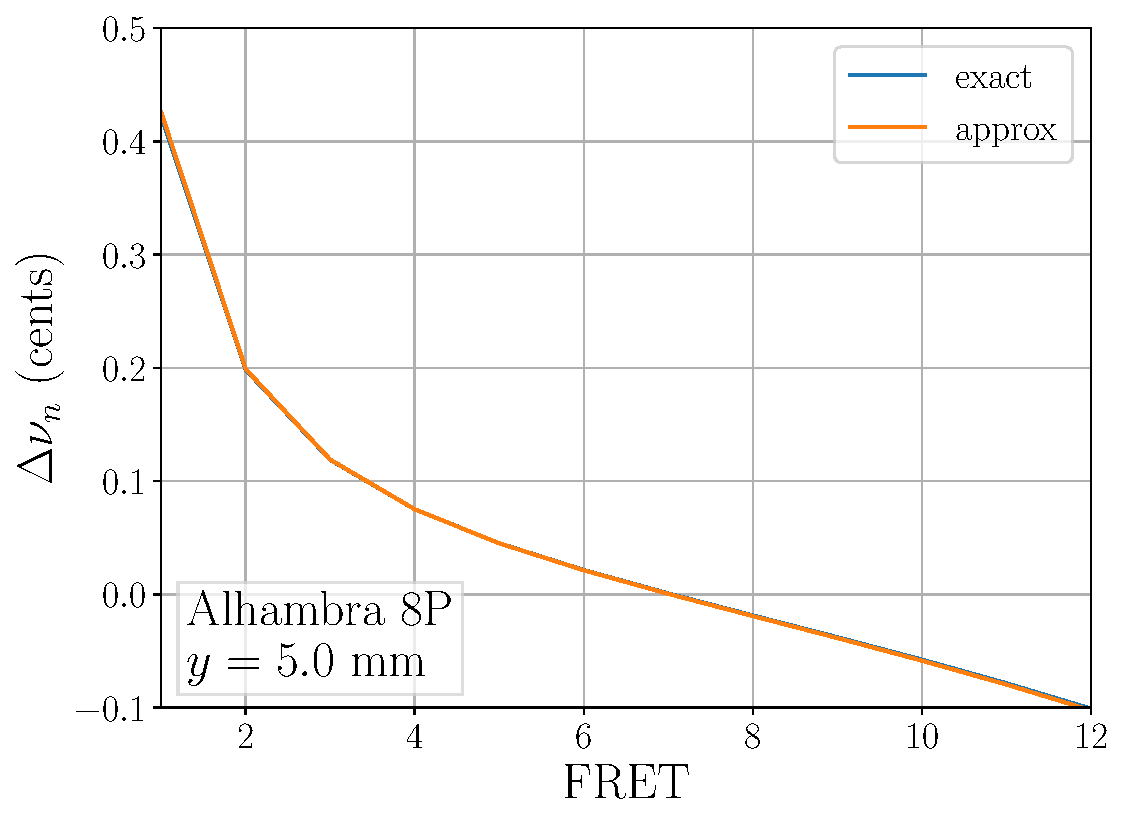
\includegraphics[width=5.0in]{figures/quad_shift_factory}
%  \caption{\label{fig:quad_shift_factory} Total frequency shift (in cents) due to resonant length and linear mass density for a transverse displacement of $y = 5$~mm. This shift is identical for each string, and should be smaller than the experimental errors we'll accumulate using our transverse displacement approach.}
% \end{figure}
%
%\begin{table}%[htbp]
%  \centering
%  \caption{\label{tbl:ej43_props} Derived physical properties of the D'Addario Pro-Arte Nylon Classical Guitar Strings -- Light Tension (EJ43). The corresponding scale length is 650 mm.}
%    \begin{tabular}{lcccc}
%    \hline \hline
%    String  & $R$ & $\kappa$ & Modulus (GPa) & Stiffness \\
%    \hline
%    J4301 & 4.39 $\times 10^{4}$ & 49.8 & 8.62 & 3.79 $\times 10^{-3}$ \\
%    J4302 & 5.02 $\times 10^{4}$ & 57.0 & 5.62 & 4.68 $\times 10^{-3}$ \\
%    J4303 & 4.79 $\times 10^{4}$ & 54.4 & 3.57 & 5.72 $\times 10^{-3}$ \\
%    J4304 & 5.02 $\times 10^{4}$ & 57.0 & 9.52 & 4.13 $\times 10^{-3}$ \\
%    J4305 & 4.39 $\times 10^{4}$ & 49.8 & 5.05 & 4.55 $\times 10^{-3}$ \\
%    J4306 & 5.27 $\times 10^{4}$ & 59.9 & 3.97 & 6.35 $\times 10^{-3}$ \\
%    \hline
%    \end{tabular}%
%  \label{tab:addlabel}%
%\end{table}%

\begin{table}%[htbp]
  \centering
  \caption{\label{tbl:ej43_props} Derived physical properties of the D'Addario Pro-Arte Nylon Classical Guitar Strings -- Light Tension (EJ43). The corresponding scale length is 650 mm.}
    \begin{tabular}{lcccc}
    \hline \hline
    String  & $R$ & $\kappa$ & Modulus (GPa) & Stiffness \\
    \hline
    J4301 & 2.67 $\times 10^{4}$ & 29.8 & 5.17 & 2.94 $\times 10^{-3}$ \\
    J4302 & 1.09 $\times 10^{4}$ & 11.6 & 1.14 & 2.11 $\times 10^{-3}$ \\
    J4303 & 6.63 $\times 10^{4}$ & 75.6 & 4.97 & 6.75 $\times 10^{-3}$ \\
    J4304 & 2.60 $\times 10^{4}$ & 29.1 & 4.86 & 2.95 $\times 10^{-3}$ \\
    J4305 & 2.66 $\times 10^{4}$ & 29.7 & 3.02 & 3.52 $\times 10^{-3}$ \\
    J4306 & 1.40 $\times 10^{4}$ & 15.2 & 1.01 & 3.20 $\times 10^{-3}$ \\
    \hline
    \end{tabular}%
  \label{tab:addlabel}%
\end{table}%


\begin{table}%[htbp]
  \centering
  \caption{\label{tbl:ej46_props} Derived physical properties of the D'Addario Pro-Arte Nylon Classical Guitar Strings -- Hard Tension (EJ46). The corresponding scale length is 650 mm.}
    \begin{tabular}{lcccc}
    \hline \hline
    String  & $R$ & $\kappa$ & Modulus (GPa) & Stiffness \\
    \hline
    J4301 & 10.2 $\times 10^{4}$ & 116.5 & 20.1 & 6.01 $\times 10^{-3}$ \\
    J4302 & 4.13 $\times 10^{4}$ & 46.7 & 4.65 & 4.37 $\times 10^{-3}$ \\
    J4303 & 2.96 $\times 10^{4}$ & 33.2 & 2.16 & 4.61 $\times 10^{-3}$ \\
    J4304 & 4.66 $\times 10^{4}$ & 52.8 & 8.47 & 4.26 $\times 10^{-3}$ \\
    J4305 & 1.79 $\times 10^{4}$ & 19.7 & 2.13 & 3.12 $\times 10^{-3}$ \\
    J4306 & 2.65 $\times 10^{4}$ & 29.6 & 1.96 & 4.68 $\times 10^{-3}$ \\
    \hline
    \end{tabular}%
  \label{tab:addlabel}%
\end{table}%

%\begin{table}%[htbp]
%  \centering
%  \caption{\label{tbl:ej45_mod} Effective Young's Modulus for the D'Addario Pro-Arte Nylon Classical Guitar Strings -- Normal Tension (EJ45). The corresponding scale length is 650 mm. \red{Note that these estimates are reasonable but not quite as credible as we'd like, particularly given the effort required to obtain them. We expect the moduli of the first three strings to be the same, but they differ by as much as 40\%.}}
%    \begin{tabular}{lc}
%    \hline \hline
%    String  & \multicolumn{1}{l}{Modulus (GPa)} \\
%    \hline
%    J4501 & 13.8 \\
%    J4502 & 10.9 \\
%    J4503 & 9.86 \\
%    J4504 & 11,3 \\
%    J4505 & 8.09 \\
%    J4506 & 5.71 \\
%    \hline
%    \end{tabular}%
%  \label{tab:addlabel}%
%\end{table}%

% \begin{figure}
%  \centering
%  \begin{subfigure}[b]{0.8\textwidth}
%   \centering
%   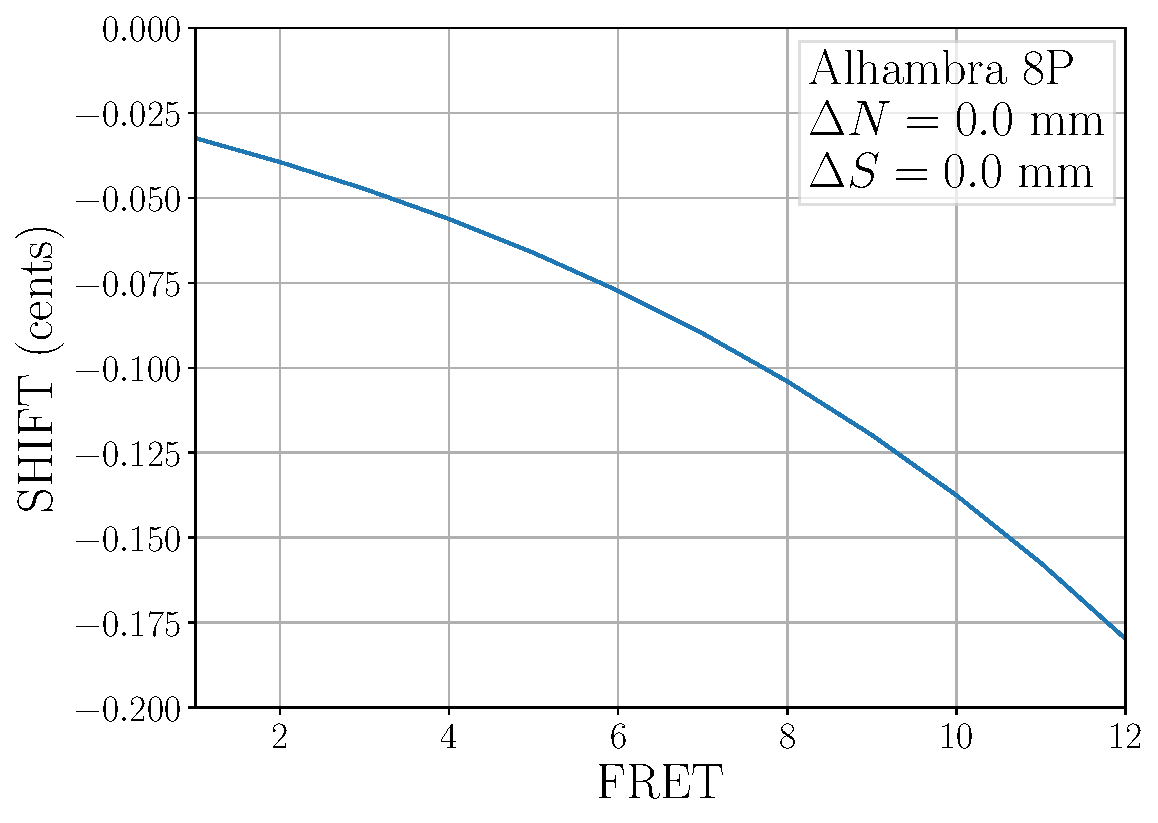
\includegraphics[width=5.0in]{figures/norm_error_uncompensated}
%   \caption{Frequency shift for an uncompensated guitar}
%   \label{fig:norm_error_uncompensated}
%  \end{subfigure}
%  \par\vspace{0.25in}
%  \begin{subfigure}[b]{0.8\textwidth}
%   \centering
%   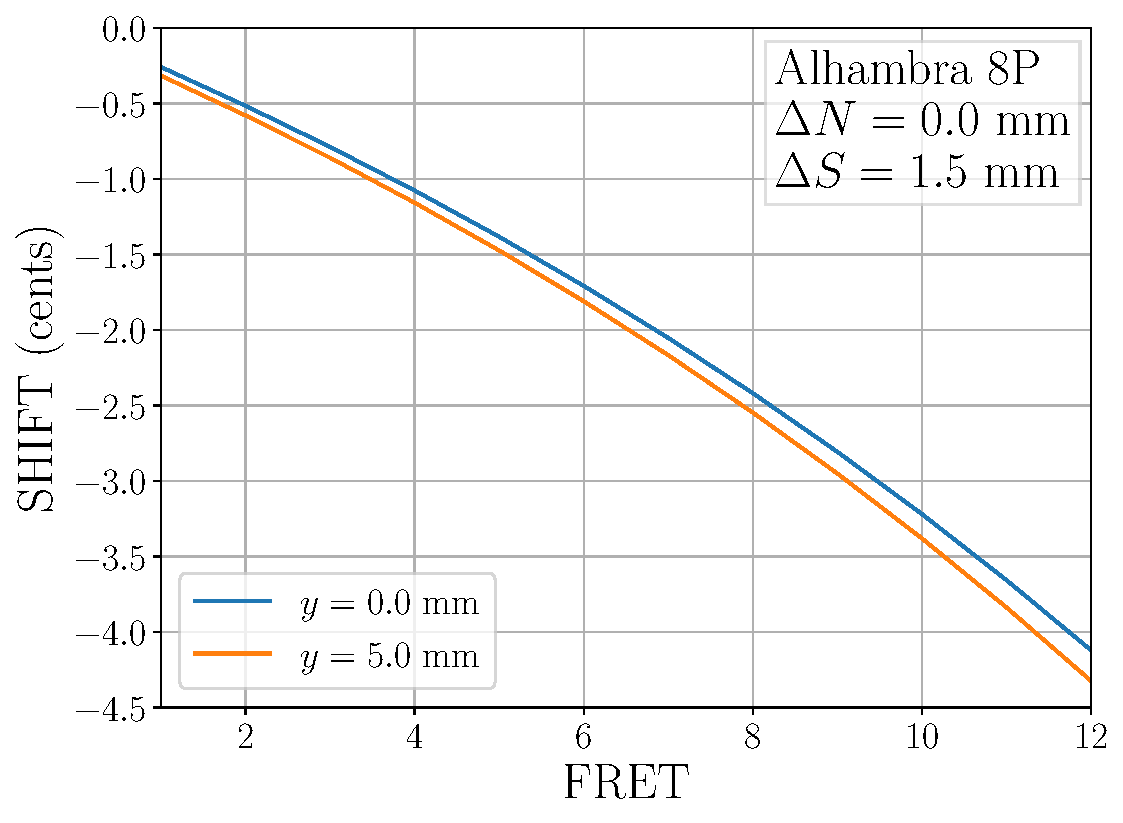
\includegraphics[width=5.0in]{figures/norm_error_factory}
%   \caption{Frequency shift for a factory guitar}
%   \label{fig:norm_error_factory}
%  \end{subfigure}
%  \caption{\label{fig:norm_error} Frequency shift (in cents) due to the fretted length $L_n$ for an uncompensated (a) and factory (b) Alhambra 8P guitar, for both zero and nonzero lateral displacement $y$.}
% \end{figure}
%
% \begin{figure}
%  \centering
%  \begin{subfigure}[b]{0.8\textwidth}
%   \centering
%   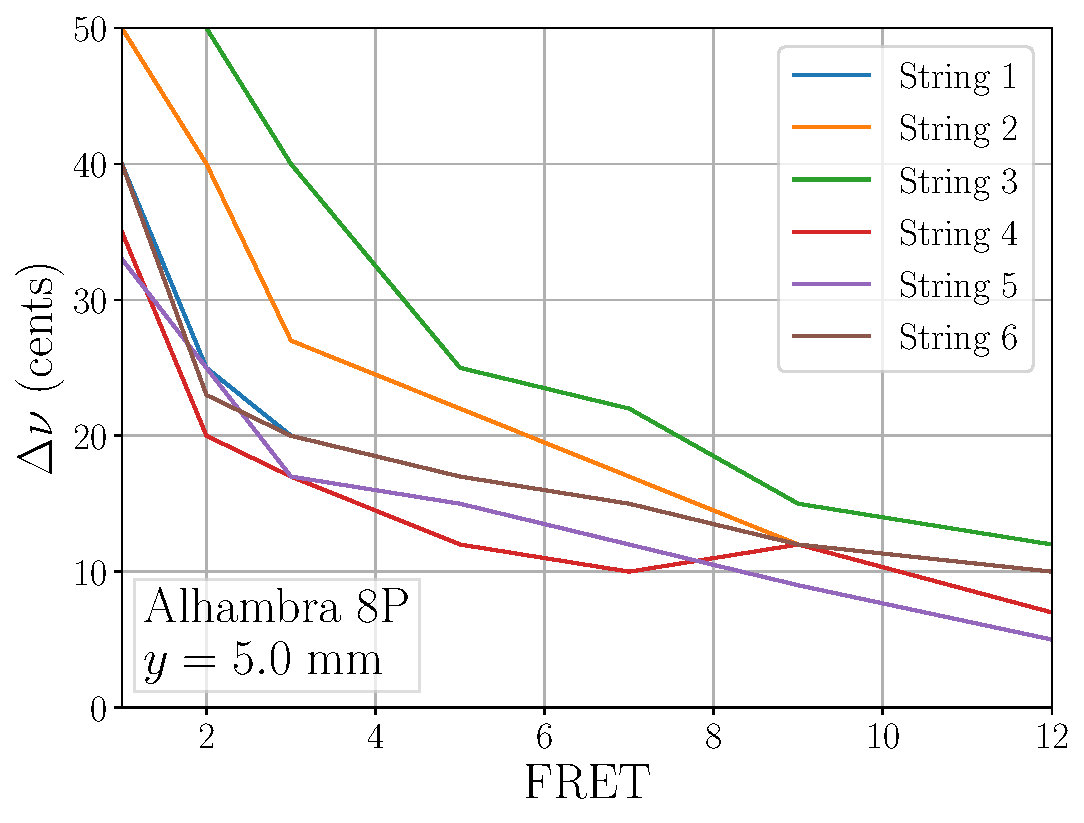
\includegraphics[width=5.0in]{figures/shift_data}
%   \caption{Experimental data}
%   \label{fig:shift_data}
%  \end{subfigure}
%  \par\vspace{0.25in}
%  \begin{subfigure}[b]{0.8\textwidth}
%   \centering
%   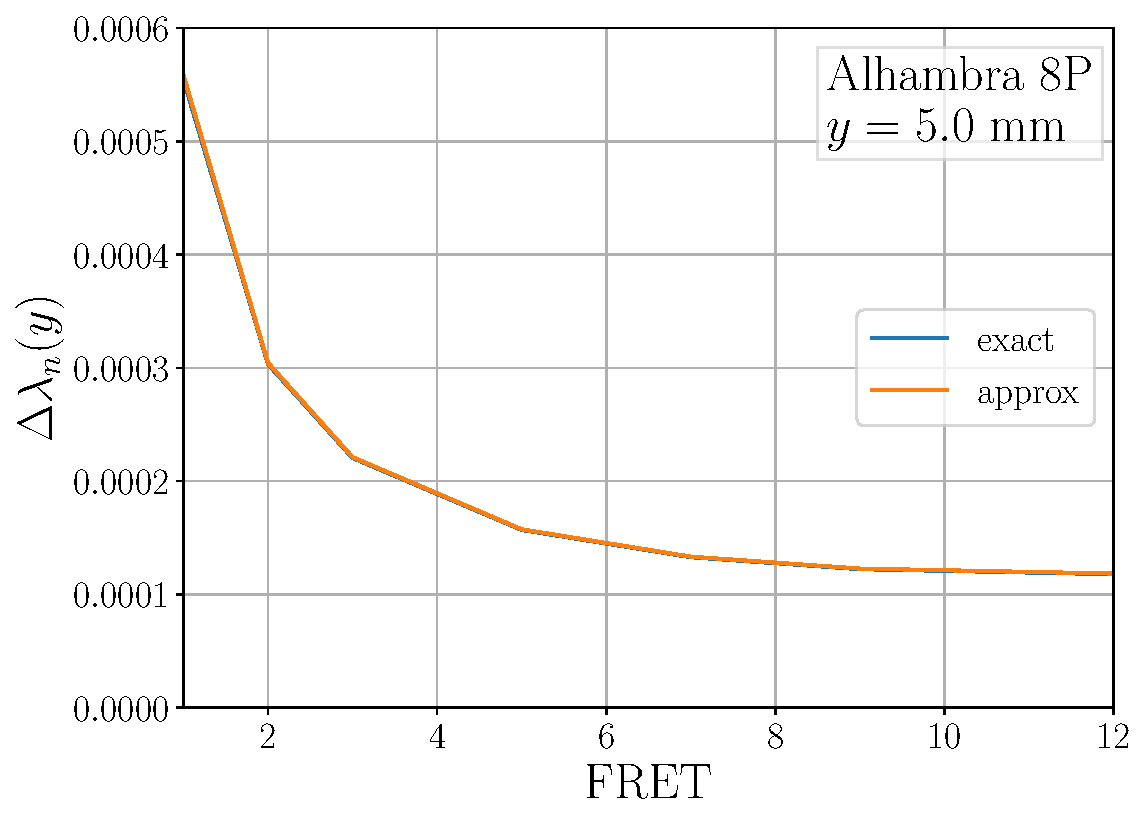
\includegraphics[width=5.0in]{figures/delta_lambda}
%   \caption{Calculated change in total string length $\mathcal{L}$}
%   \label{fig:delta_l}
%  \end{subfigure}
%  \caption{\label{fig:exp_data} Frequency shift (in cents) (a) and change in total string length $\mathcal{L}$ (b) due to lateral displacement $y$.}
% \end{figure}
